% !TEX root = main.tex

% TODO:
% REMARK:

\section{CP Asymmetry in Top quarks pair and corresponding observables/models}
\label{sec:AcpModelObs}

	With the real 2016 data from CMS, a complete analysis on $t\bar{t}$ CPV is done and mentioned in previous chapters. The analysis focuses on the CPV probable coming from the $t\bar{t}$ in CEDM model and it uses the triple products to be the CP observable to do the measurement on the data. However, there are not only triple products' type observable could be used, but also another type which is characterized as T-even observables; There are also not only CEDM model could be the source of top quarks' CPV, but 2HDM model which has been discussed since decades. 

	\subsection{Models}
	\label{ssec:AcpModel}

		In reference \cite{Atwood:2000tu}, it is particularly organized the information about CPV in top quarks. The usual discussions about CPV in top quarks are related to CEDM model and 2HDM model.

		\subsubsection{ CEDM model}
		\label{sssec:AcpModel_CEDM}



			The CEDM model's asymmtry from real part of $d_t^g$ could be detected by T-odd observables only, and imagininary part of $d_t^g$ could be detected by T-even observables.(T-odd and T-even will be menntioned in section\ref{ssec:AcpObs}) However, the implementation to generate the model lagrangian with program FeynRules(cite****), the imaginary part of $d_t^g$ is not allowed inputting. Now, therefore, the MadGraph generator we use could not make CEDM sample with imaginary part of $d_t^g$. If there will be hacked into the FeynRules and successfully imsert the restricted imaginary part now, the T-even observable behavior corresponding to $Im(d_t^g)$ will be still an interesting issue.

		\subsubsection{ 2HDM model}
		\label{sssec:AcpModel_2HDM}

			The only detected neural Higgs-boson in standard model is CP and flavor conserving automatically. However, the extended Higgs sector could be allowed feature of  CP violation. The beyond standard model's 2HDM model is the probable case and one of simple case of Higgs sector with CP violation. For the top quark, because of it's heavy mass, the larger effect of CPV is expected in the Higgs sector. It is known that 2hDM extensions with natural flavour conservation at the tree level and explicit CP violation are by complex Yukawa coupling matrices which lead to a Kobayashi-Maskawa (KM) phase, and also by tree level Higgs potential V($\Phi_1$, $\Phi_2$). CP violation in the scalar potential induces blending of CP–even and –odd scalars, and in this way leading to 3 mass eigenstates but not CP eigenstates, so we have couplings:

			\begin{equation}
			\begin{split}
			L_Y = -(\sqrt{2} G_F)^{1/2}\sum_{j,f}^{}m_f(a_{jf}\bar{f}f + \~{a}_{jf} \bar{f} i \gamma_5 f)\phi_j
			\label{eq:2HDM_scalar}
			\end{split}
			\end{equation}
			\FloatBarrier

			where the $G_F$ is Fermi’s constant, f presents a quark/lepton field and $m_f$ its associated mass, and $a_{jf}$ , $\~{a}_{jf}$ are the reduced (pseudo)scalar Yukawa couplings. The couplings are related to parameters of the scalar potential. And for the top quark:

			\begin{equation}
			\begin{split}
			L_Y = -(\sqrt{2} G_F)^{1/2}\sum_{j=1}^{3}m_f(a_{jt}\bar{f}f + \~{a}_{jt} \bar{f} i \gamma_5 t)\phi_j \;\;\;\;\;\;\;\;\;\;\;\;\;\;\;\;\\
			a_{jt} = d_{2j}/\sin{\beta} \; \; , \; \; \; \; \; \~{a}_{jt} = -d_{3j}\cot{\beta} \; \; , \; \; \; \; \; \tan{\beta} = v_2/v_1
			\label{eq:2HDM_scalar_t}
			\end{split}
			\end{equation}
			\FloatBarrier

			$v_1$, $v_2$ are the vacuum expectation values of the two doublets, and $d_{2j}$, $d_{3j}$ are the matrix elements of a 3×3 orthogonal matrix which describes the mixing of the neutral states. To do the measurement of CPV in flavor–diagonal reactions like $gg \rightarrow t\bar{t}$, $qq^- \rightarrow t\bar{t}$ is:

			\begin{equation}
			\begin{split}
			\gamma_{cp} = -a \widetilde{a} = d_{2j}d_{3j}\cot{\beta}/\sin{\beta}
			\label{eq:2HDM_rawCPV}
			\end{split}
			\end{equation}
			\FloatBarrier

			Futhermore, the CP violation in the Higgs sector can be evoked in the model where the coupling in the Higgs potential is complex. The complex coupling may cause the CP-violating interaction directly, and the complex VEV(vacuum expectation value)'s of of Higgs field that could contain CPV effect. Also, the real potential could lead to a ground state in which CP breaks spontaneously. The tree-level Higgs potential of 2HDM model is shown below:(Eq.\ref{eq:2HDM_potential})

			\begin{equation}
			\begin{split}
			V(\Phi_1, \Phi_2) = -\mu^2_{11} \Phi^{\dagger}_{1}\Phi_{1} -\mu^2_{22} \Phi^{\dagger}_{2}\Phi_{2} - ( \mu^2_{12} \Phi^{\dagger}_{1}\Phi_{2} + h.c.) \\
			+ \lambda_1(\Phi^{\dagger}_{1}\Phi_{1})^2 + \lambda_2(\Phi^{\dagger}_{2}\Phi_{2})^2 + \lambda_3(\Phi^{\dagger}_{1}\Phi_{1}\Phi^{\dagger}_{2}\Phi_{2}) + \lambda_4(\Phi^{\dagger}_{1}\Phi_{2})(\Phi^{\dagger}_{2}\Phi_{1})\\
			+ \frac{1}{2}[\lambda_5(\Phi^{\dagger}_{1}\Phi_{2})^2 + h.c. ] + [ \lambda_6 \Phi^{\dagger}_{1}\Phi_{1}\Phi^{\dagger}_{1}\Phi_{2} + \lambda_7 \Phi^{\dagger}_{2}\Phi_{2}\Phi^{\dagger}_{2}\Phi_{1} + h.c.]
			\label{eq:2HDM_potential}
			\end{split}
			\end{equation}
			\FloatBarrier

			The particle spectrum of 2HDM model are three neutral Higgs-bosons and 2 charged Higgs-bosons which are denoted by $H^{k}$(k=1,2,3) and $H^{+(-)}$. The key parameters of 2HDM model which could lead to CP violation in the Higgs sector are $\lambda_5$, $\lambda_6$, $\lambda_7$, and $\mu_{12}^2$, and there are some organized scenario from \cite{Atwood:2000tu} --

			\begin{itemize}
				\item 
				\item
				\item
				\item
			\label{AcpModelObs:itm:4_sce_of_2HDM}
			\end{itemize}

			The previous organization and more 2HDM model and parameters discussion would be in the refernce of particle-phenomenology papers \cite{Atwood:2000tu}, \cite{ElKaffas:2006gdt}, \cite{Khater:2003wq}, \cite{Keus:2015hva}, \cite{Iguro:2019zlc}, \cite{Bernreuther:1993hq}, \cite{Bernreuther:1998qv}.

			2HDM model's CPV could be detected by CP-odd observables with both T-odd or T-even property according to the derivation (ref 1993derivation). Because the parameters in 2HDM model is too comlicated to tune, it is not the bottom line of us to approach. There will be done by some fundamental test of default parameter setting in the section.\ref{ssec:AcpObs} with various observables.



	\subsection{Observables}
	\label{ssec:AcpObs}

		The probed observables are roughly classified to two type. The first one is the CP-odd observables which is T-edd and the other is CP-odd observable which is T-even. The even/odd means the $\hat{CP}$/$\hat{T}$ operator's eigenstate with eigenvalue $+1$ and $-1$ corresponding to even and odd. 

		The triple product type observable(for example, the $O_{3,6,12,14}$ we use in the 2016 analysis) is T-odd observable.

		\subsubsection{Classification and Test}
		\label{sssec:AcpObs_class_test}

		The following testing are based on some simulation sample of $t\bar{t}$ by generator Madgraph to generate parton-level's event-by-event sample. And the showering and detector simulation would be done by Pythia cite**** and Delphes cite****.

		At first, following the paper\cite{Hayreter:2015ryk}'s(which is the basic of 2016 analysis) selection and model implementation, we also use Madgraph\cite{Alwall:2011uj} generator as it to generate $t\bar{t}$ sample of CEDM model to double-check the triple product observables action under CEDM model. The $O_{3}$, $O_{6}$, $O_{12}$, $O_{14}$ would be tested:

		\begin{figure}[H]
		\centering
		    \subfigure[$O_{3}$]{\includegraphics[width=0.45\textwidth]{Figures/Observables/O_{3}.pdf}}
		    \subfigure[$O_{6}$]{\includegraphics[width=0.45\textwidth]{Figures/Observables/O_{6}.pdf}}\\
		\end{figure}
		\FloatBarrier
		\begin{figure}[H]
		\centering
		    \subfigure[$O_{12}$]{\includegraphics[width=0.45\textwidth]{Figures/Observables/O_{12}.pdf}}
		    \subfigure[$O_{14}$]{\includegraphics[width=0.45\textwidth]{Figures/Observables/O_{14}.pdf}}\\
		\caption{Reproduction of the results from \cite{Hayreter:2015ryk}}
		\label{Obs:fig:reproduce}
		\end{figure}
		\FloatBarrier


		Also, we also test that the asymmetry of standard model, CEDM model($d_t^g=5$),and 2HDM model(default parameters setting\cite{2HDM_NLO_UFO}) in parton level by Madgraph generator to see the four triple product observables acting under these models.

		\begin{figure}[H]
		\centering
		    \subfigure[SM, Muon channel]{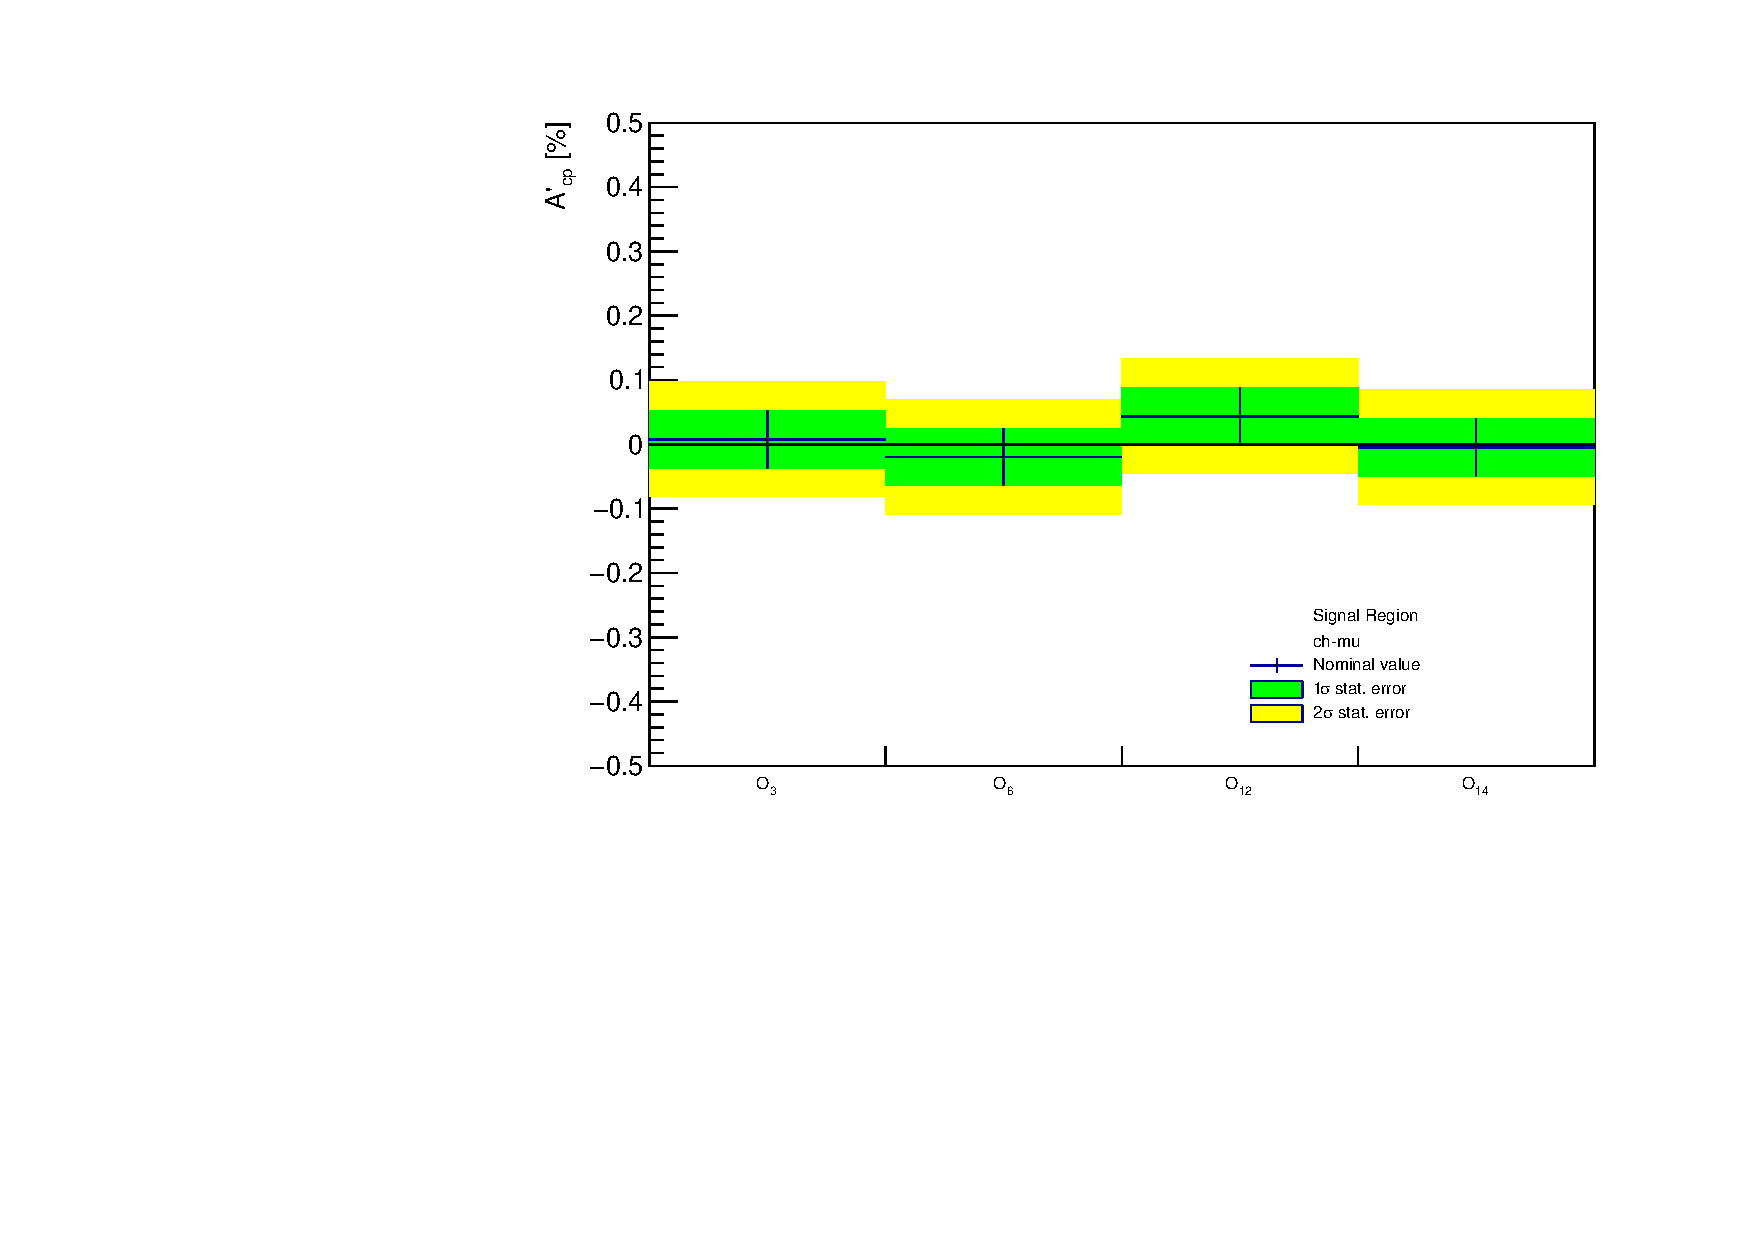
\includegraphics[width=0.45\textwidth]{Figures/Observables/TP_doublecheck/Acp_TP_semilep_genAcp_NoSel_10_7-semi_SM_i5_0j_mu.pdf}}
		    \subfigure[SM, Electron channel]{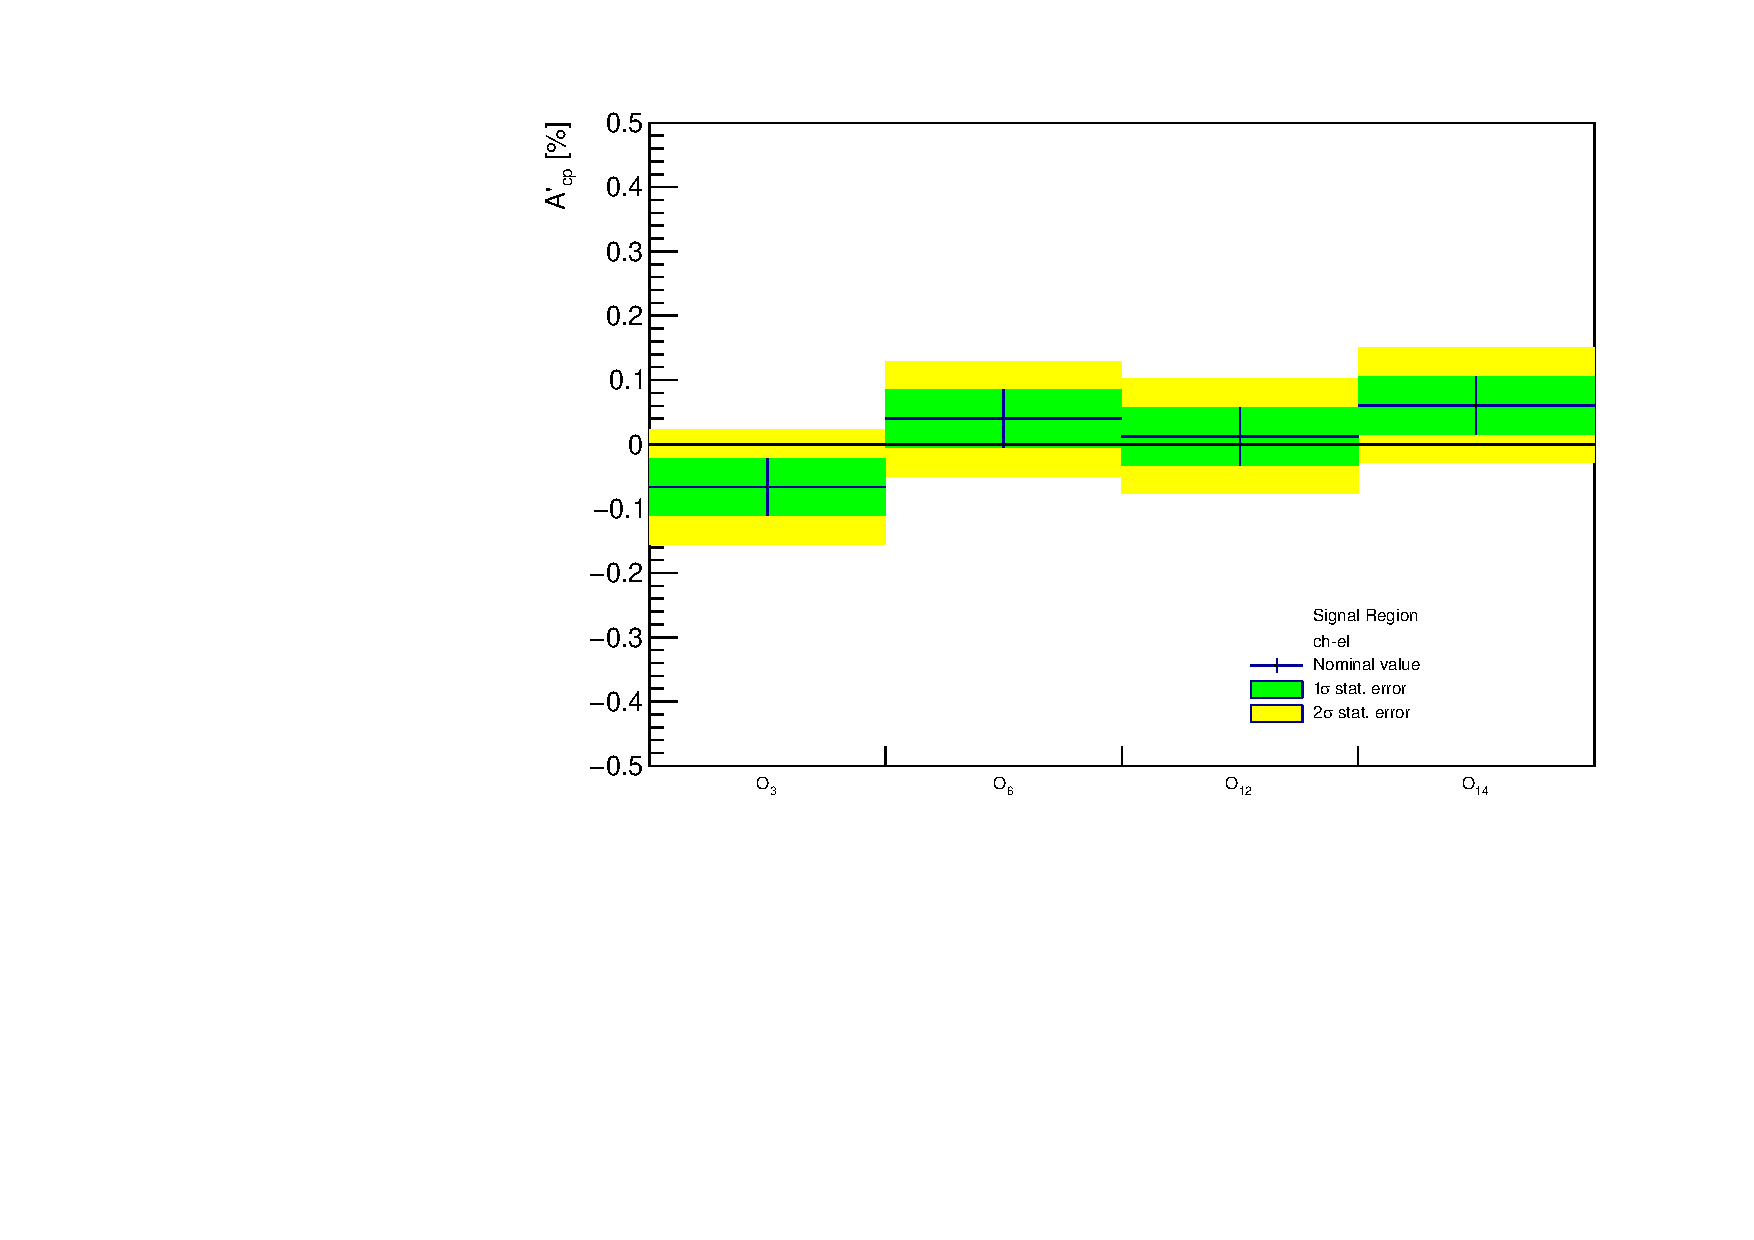
\includegraphics[width=0.45\textwidth]{Figures/Observables/TP_doublecheck/Acp_TP_semilep_genAcp_NoSel_10_7-semi_SM_i5_0j_el.pdf}}\\
		\end{figure}
		\FloatBarrier
		\begin{figure}[H]
		\centering
		    \subfigure[CEDM, Muon channel]{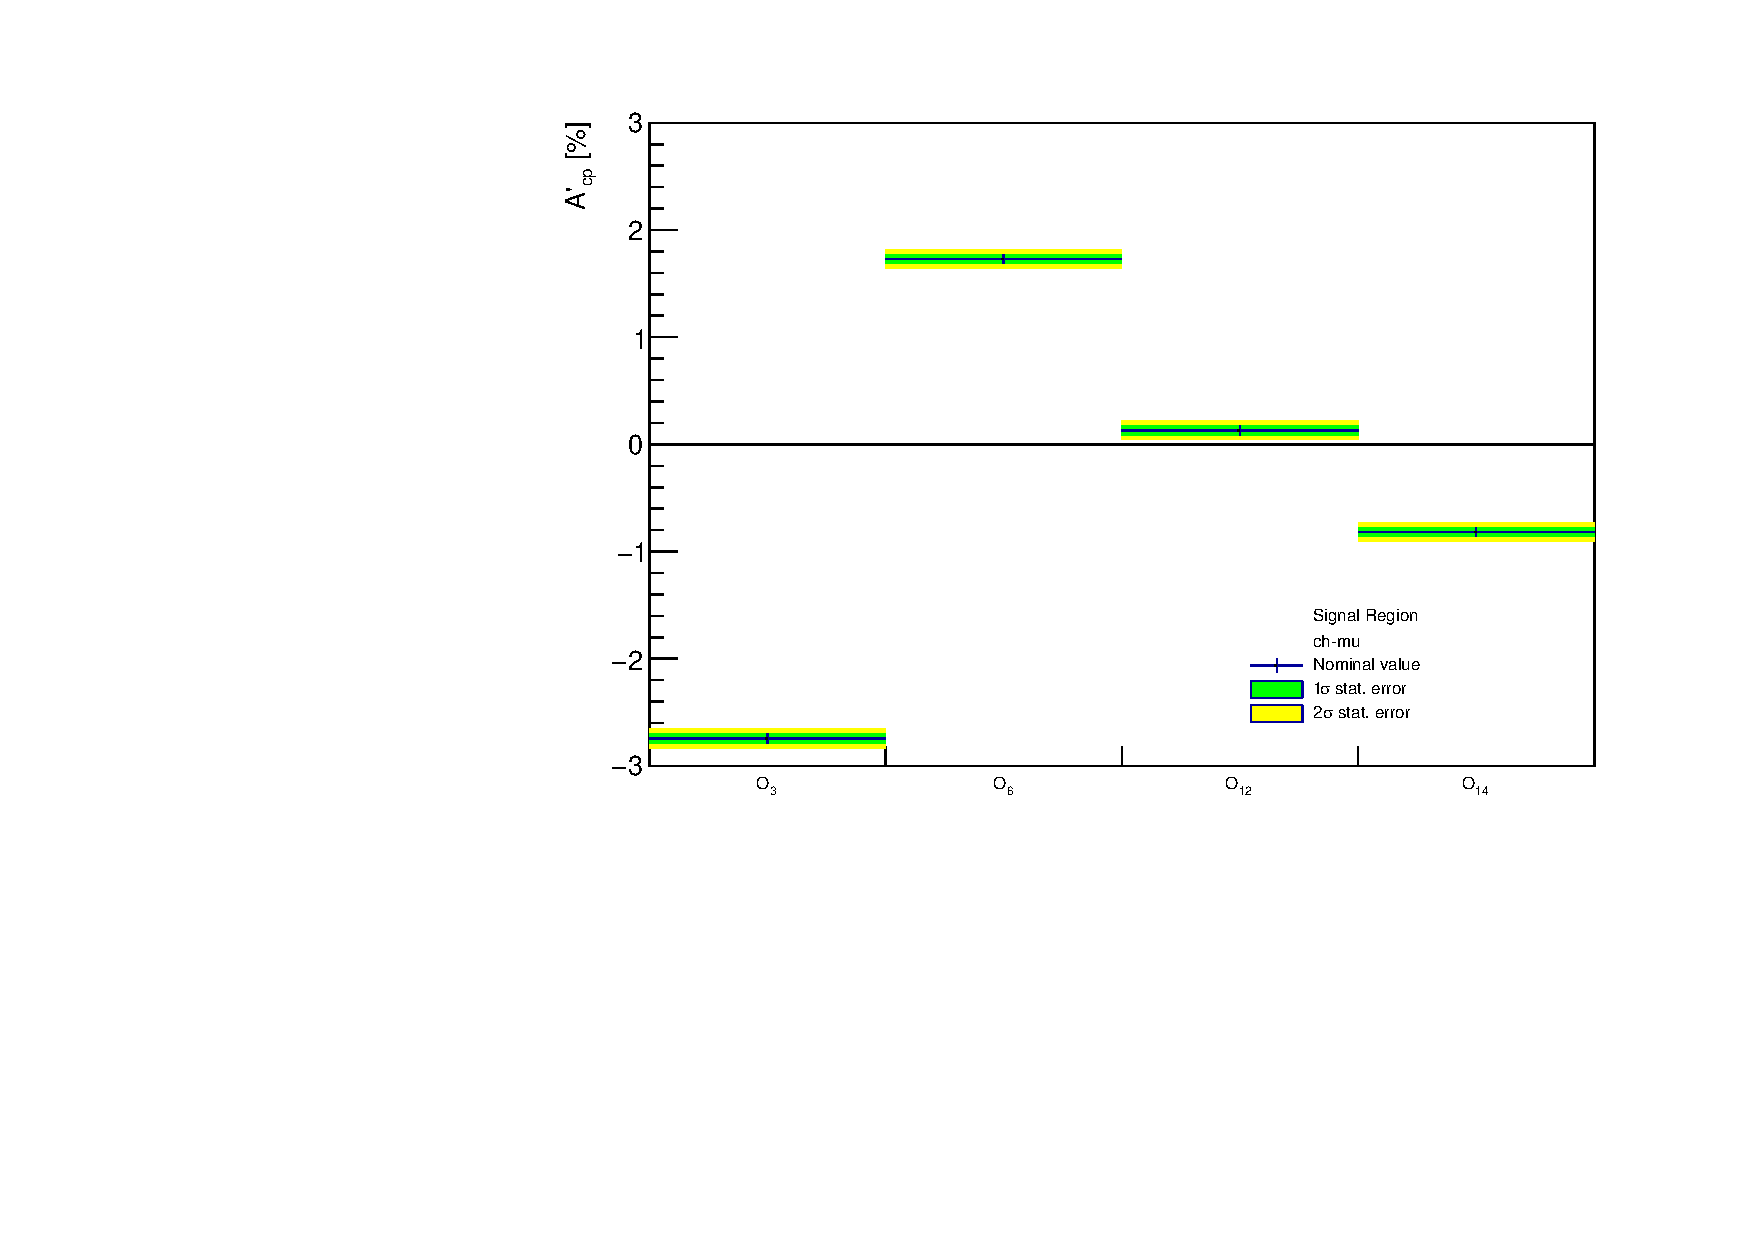
\includegraphics[width=0.45\textwidth]{Figures/Observables/TP_doublecheck/Acp_TP_semilep_genAcp_NoSel_10_7-semi_CEDM5_0j_mu.pdf}}
		    \subfigure[CEDM, Electron channel]{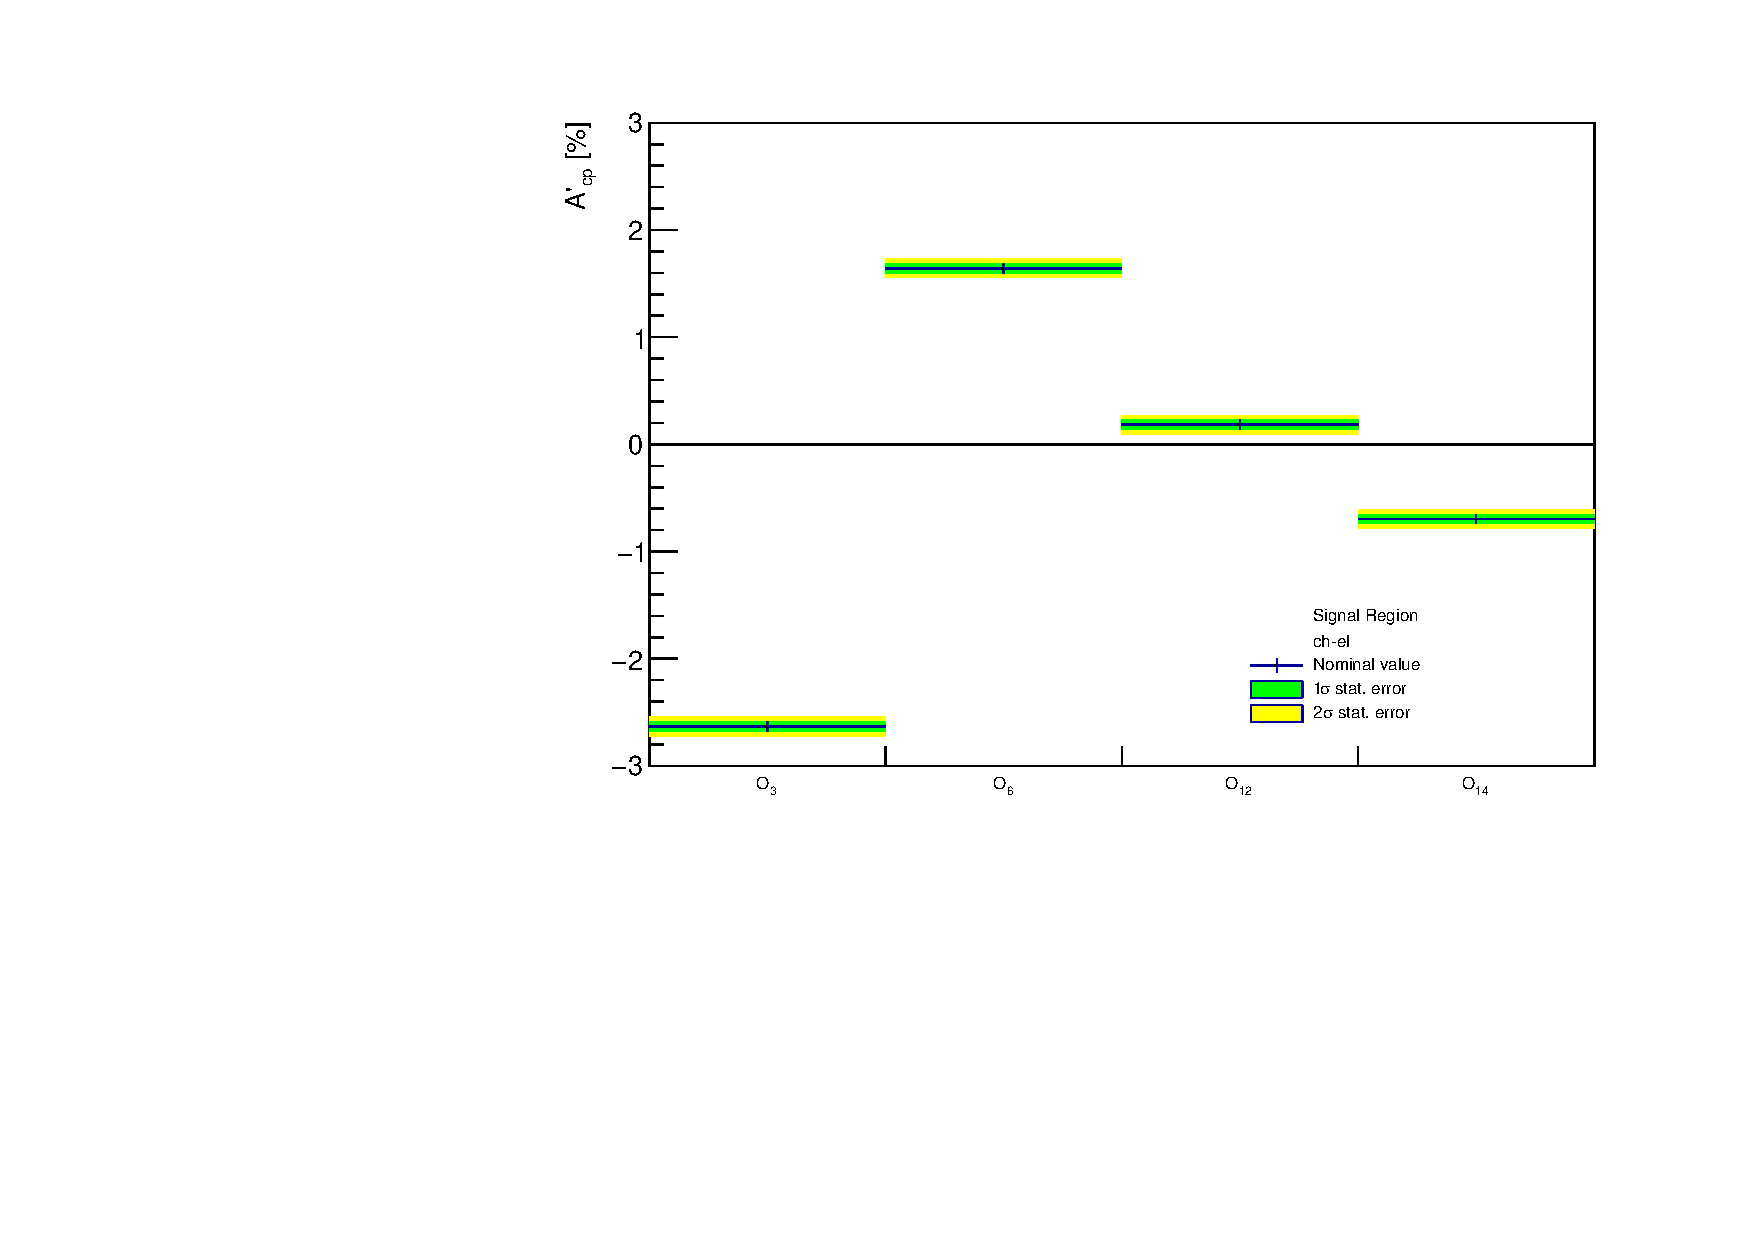
\includegraphics[width=0.45\textwidth]{Figures/Observables/TP_doublecheck/Acp_TP_semilep_genAcp_NoSel_10_7-semi_CEDM5_0j_el.pdf}}\\
		\end{figure}
		\FloatBarrier
		\begin{figure}[H]
		\centering
		    \subfigure[2HDM, Muon channel]{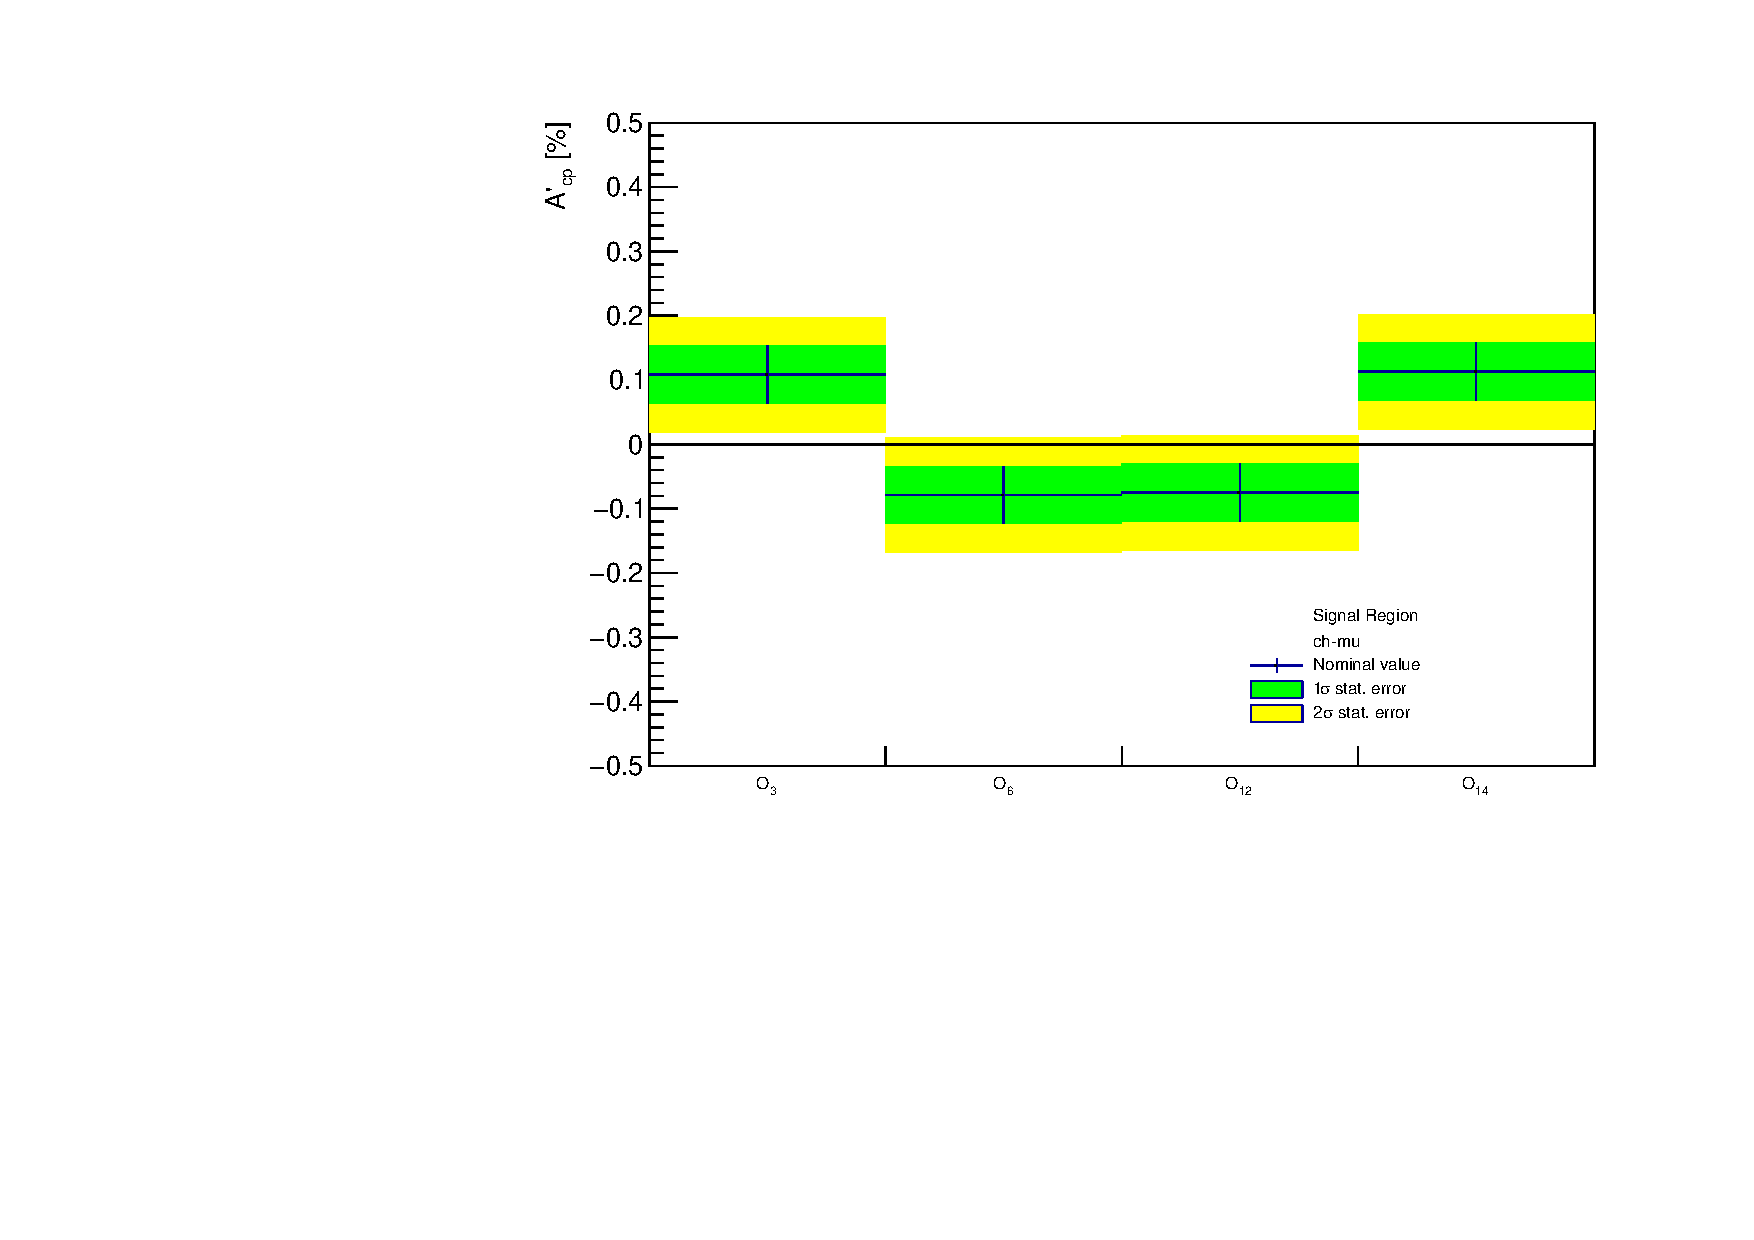
\includegraphics[width=0.45\textwidth]{Figures/Observables/TP_doublecheck/Acp_TP_semilep_genAcp_NoSel_10_7-semi_2HDM_NLO_m1_0j_mu.pdf}}
		    \subfigure[2HDM, Electron channel]{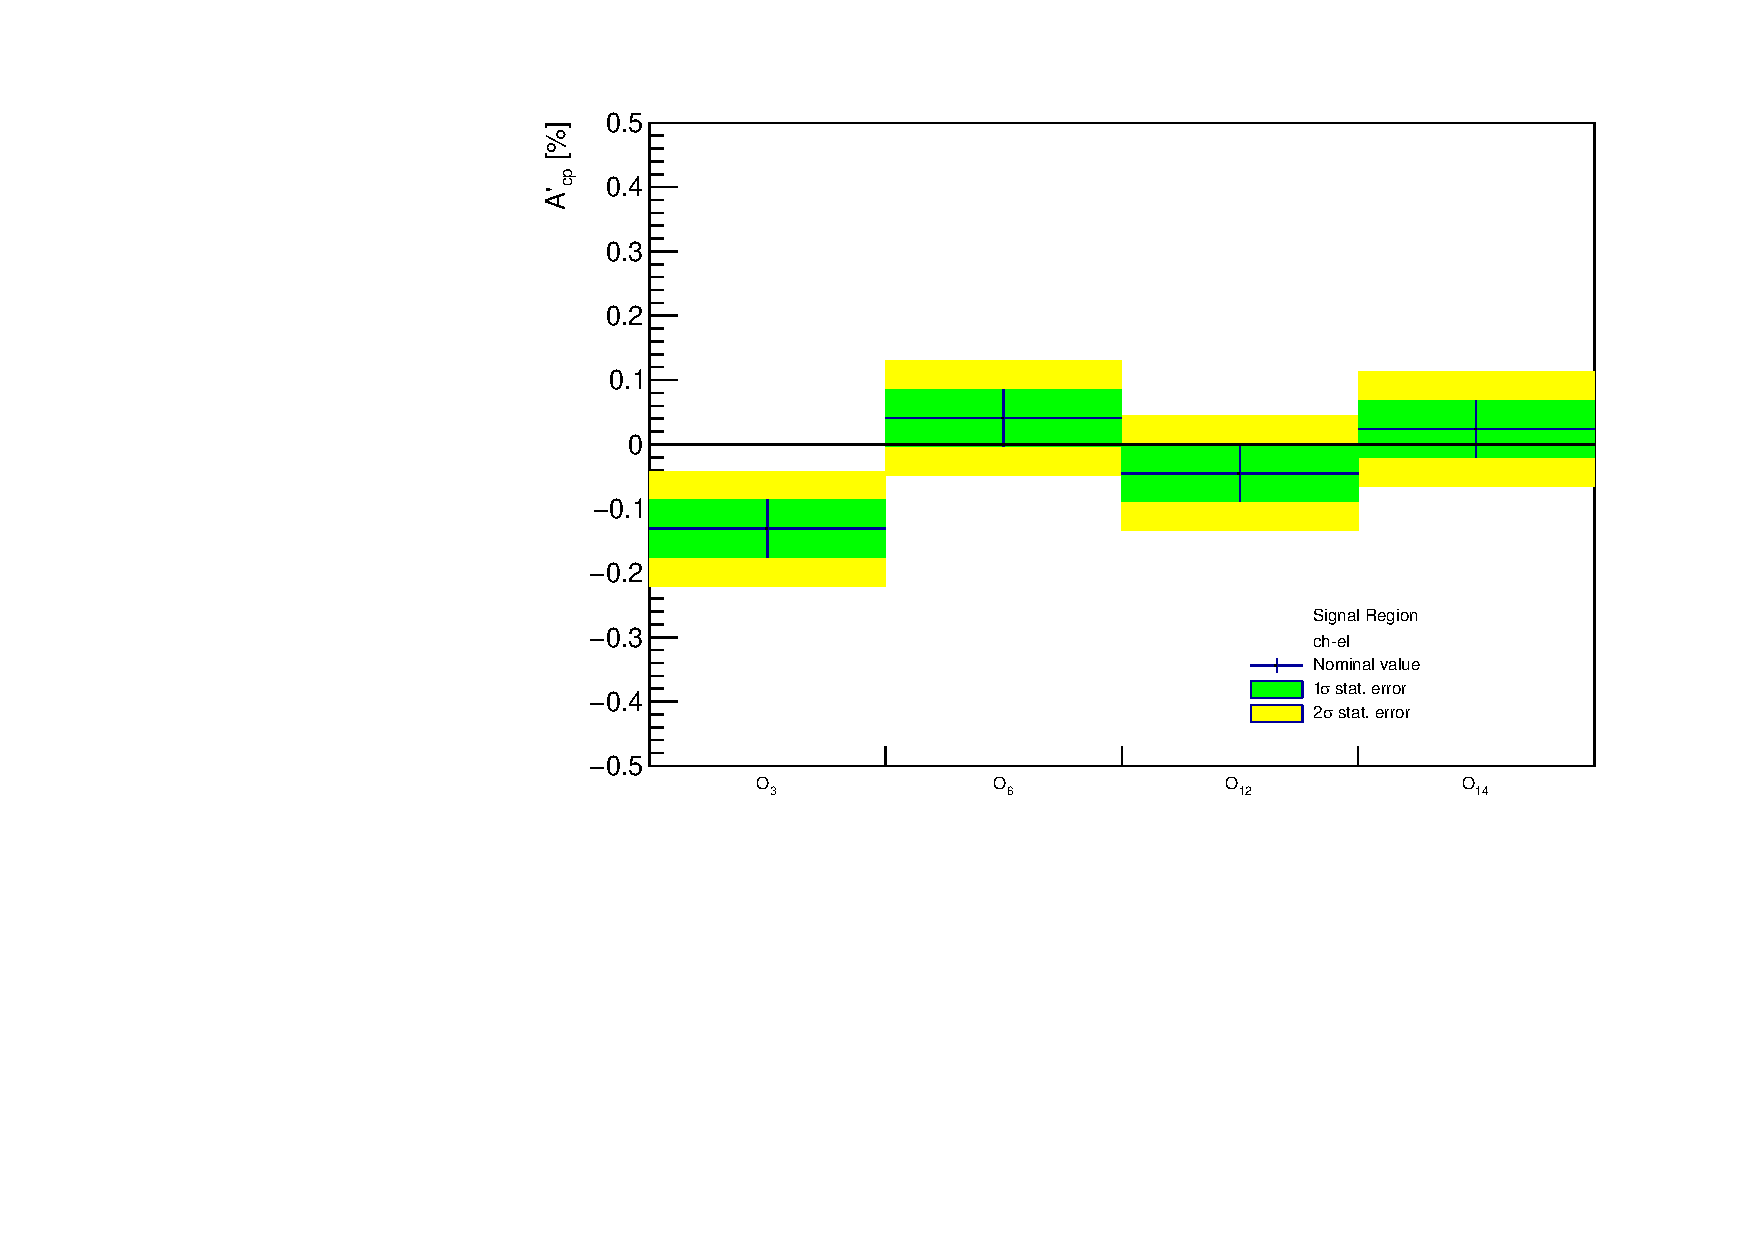
\includegraphics[width=0.45\textwidth]{Figures/Observables/TP_doublecheck/Acp_TP_semilep_genAcp_NoSel_10_7-semi_2HDM_NLO_m1_0j_el.pdf}}\\
		\caption{Measurement of three model's(SM, CEDM with $d_t^g=5$, 2HDM with default parameters setting) simulation sample with four triple product observables}
		\label{Obs:fig:TP_3model}
		\end{figure}
		\FloatBarrier

		Compared to the standard model's results -- the asymmetry values are supposely drop into 2 standard deviation range, the CEDM model shows great sensitivity to the triple product observables, and the 2HDM model with default parameter setting shows a little probability to be detect.

		Because of the extensive usage of triple-product-type observables, which is roughly equal to T-odd observales, to measure the asymmetry in $t\bar{t}$, we put emphasis on T-even observable here.

		% Peskin

		% B&B 1993

		% B&B 1998

		% revised Peskin


		% T-even 1998b&b p.5~7 could be the origin of T-even observable's design concept.

		\subsubsection{Observable property}
		\label{sssec:AcpObs_property}


\FloatBarrier
